%
% File acl2020.tex
%
%% Based on the style files for ACL 2020, which were
%% Based on the style files for ACL 2018, NAACL 2018/19, which were
%% Based on the style files for ACL-2015, with some improvements
%%  taken from the NAACL-2016 style
%% Based on the style files for ACL-2014, which were, in turn,
%% based on ACL-2013, ACL-2012, ACL-2011, ACL-2010, ACL-IJCNLP-2009,
%% EACL-2009, IJCNLP-2008...
%% Based on the style files for EACL 2006 by
%%e.agirre@ehu.es or Sergi.Balari@uab.es
%% and that of ACL 08 by Joakim Nivre and Noah Smith

\documentclass[11pt,a4paper]{article}
\usepackage[hyperref]{acl2020}
\usepackage{times}
\usepackage{latexsym}
\renewcommand{\UrlFont}{\ttfamily\small}
\usepackage{amsmath}

% This is not strictly necessary, and may be commented out,
% but it will improve the layout of the manuscript,
% and will typically save some space.
\usepackage{microtype}
\usepackage{graphicx} %package to manage images
\usepackage{caption}
\usepackage{subcaption}
\graphicspath{ {images/} }

\aclfinalcopy % Uncomment this line for the final submission
%\def\aclpaperid{***} %  Enter the acl Paper ID here

%\setlength\titlebox{5cm}
% You can expand the titlebox if you need extra space
% to show all the authors. Please do not make the titlebox
% smaller than 5cm (the original size); we will check this
% in the camera-ready version and ask you to change it back.

\newcommand\BibTeX{B\textsc{ib}\TeX}

\title{Encoding Spatial Relations from Natural Language}

\author{Mohamed Zarzoura}

\date{}

\begin{document}
\maketitle

\begin{abstract}

 In Natural language processing (NLP) space, deep neural networks (NNs) successfully provide compositional representations of words and complex linguistic units. However, there is still an improvement in the area related to spatial language. Spatial language understanding is crucial in many applications
 that need language grounding in a physical world, such as dialogue systems, conditioning driving, robots, etc. In this project,  I will try to build a system capable of processing textual spatial language from a particular perspective and converting it to a different perspective. The work is based on the DeepMind paper \cite{ramalho2018encoding}.
\end{abstract}

\section{Introduction}

\begin{figure*}[t]
    \centering
    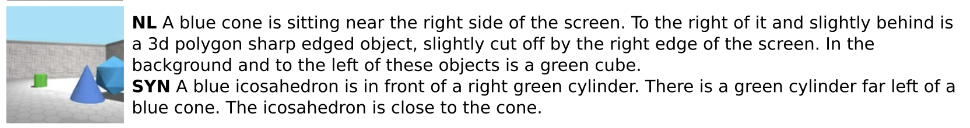
\includegraphics[width=\textwidth]{SLIMExample.png}
    \caption{example for a scene image view and its description. \textbf{[NL]} for natural language \textbf{[SYN]} for synthetic language. Taken from \cite{ramalho2018encoding}}
    \label{fig:SLIMDATA}
\end{figure*}

Spatial language involves words and phrases describing objects' position, orientation, movement, and relationships in space. Examples of spatial language include terms such as "above," "below," "near," "far," "left," "right," "up," "down," and "through." These words are often used to describe the location or movement of objects in relation to other objects, such as when we say that an object is "above" another object or is "moving to the right" or "through" another object.

Spatial language is an important aspect of human communication, as it allows us to describe and understand the world around us. For example, when we see a car moving, we might describe its movement using spatial language, saying that the car is moving "backward" or "forward." This allows us to communicate our observations clearly and helps us understand the spatial relationships between objects in the world around us. For example, we can describe the spatial properties of the moving car by saying the car on "the far left lane" is moving "forward".

In the field of artificial intelligence and natural language processing, spatial language is an important area of study. Researchers are developing algorithms and models that can understand and process spatial language, to improve the ability of computers and other machines to interpret and respond to natural language inputs. This has applications in language translation, image captioning, and spatial reasoning for machines.

Deep neural network (DNN) models have proven successful in many natural language tasks. Their success is due to their ability to represent words and other complex linguistic structures in a distributed manner. However, as shown in the baseline experiments in the GOA dataset, DNNs fail to deal with tasks that need spatial language understanding \cite{hudsonGQANewDataset2019}. These results indicate that there are  areas of improvement in natural language understanding (NLU), and spatial language understanding is one of them.

The paper "Encoding Spatial Relations from Natural Language" presents a system capable of capturing the semantics of spatial relations from natural language descriptions \citet{ramalho2018encoding}. The system uses a multi-modal objective to generate images of scenes from their textual descriptions. A new dataset was proposed for this reason. The internal representations are shown to be robust to meaning-preserving transformations of descriptions (paraphrase invariance; "a young woman in front of an old man" and "an old man behind a young woman."), and viewpoint invariance (changing of camera angle) is an emergent property of the system. The paper also introduces a large dataset of 3D scenes coupled with language descriptions from different viewpoints for training and evaluating the model.

The authors demonstrate the effectiveness of this approach by generating images from angles not seen in the training data and showing that they correspond to language descriptions of the same scene from the new angle. They also show that the learned representations align well with human similarity judgments of scene descriptions.

Overall, the paper presents an approach to learning spatial relations from language that can capture the invariances necessary for a human-like understanding of spatial descriptions. This is an important step towards building more human-like natural language processing systems.


\section{Materials and methods}

\subsection{The SLIM Dataset}

\citet{ramalho2018encoding} propose the SLIM multimodel dataset consisting of spatial textual descriptions grounded in 3D images generated from ten million scenes. Dataset scenes are about two or three colored 3D objects in a room. Each scene has ten 3D images rendered from ten different random camera angles with a textual description for each rendered image which is syntactically generated. 

Five thousand six hundred four scenes randomly selected from the ten million scenes form a smaller subset. This smaller dataset is called "natural language data," as humans provide the spatial textual description for each scene's view. In this project, I used "natural language data" (See Figure \ref{fig:SLIMDATA} taken from \citealt{ramalho2018encoding}).

\subsection{The original SLIM model}


\begin{figure*}[hbt]
    \centering
    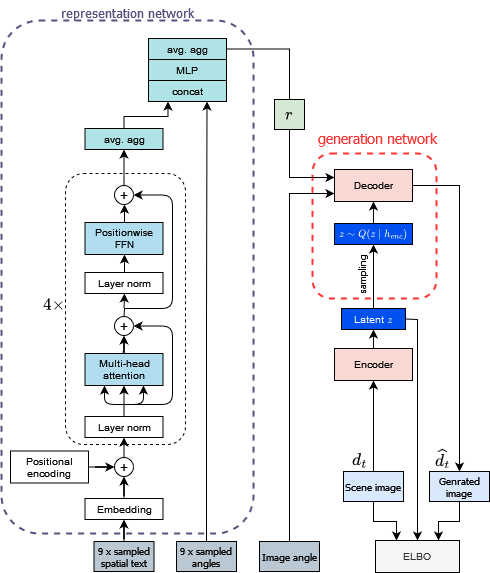
\includegraphics[width=.7\linewidth]{SLIMModel.png}
    \caption{My implementation of the Slim Model}
    \label{fig:SLIMModel}
\end{figure*}

The model consists of two parts; the first is a representation network that creates a learned "scene representation" vector by encoding several textual descriptions and their respective view angles. The second part is  a generation network that generates images conditioned on the learned scene representation and a new view angle not seen by the representation network.

\paragraph{The representation network} consists of a CNN-based language encoder followed by a layer normalization to encode the sequence of the embedded textual descriptions. The encoded sequence features are then merged using a mean aggregation function to produce a "sentence" encoding. A single-layer perceptron encodes the respective view angles. The angles and textual encoding are combined using a three-layers perceptron to create a learned vector representation per text-angle pair. A mean aggregation function merges the text-angle pair features to produce a single "scene representation" vector $r$.

\paragraph{The generation network} is a conditional RNN variational auto-encoder that uses a convolutional LSTM cell \cite{2016arXiv160408772G}. The generation network is trained using a sampled scene image $d_t$ and its camera angle $c_t$ that the representation network has not seen. The "scene representation" vector "$r$ and the image angle $c_t$ conditioned the image reconstruction from the latent space $z$ where $\hat{d_t} = g(z, c_t, r) \approx d_t, q(z|d_t) = e(d_t)$.

\subsection{The implemented SLIM model}

In my implementation, I made the following changes; the implemented model is shown in Figure \ref{fig:SLIMModel}: 

\subsubsection{The Language Encoder}

I replaced the CNN language encoder with a transformer encoder. I use the transformer because it can contextualize the tokens' encoding and considers the tokens' order. By doing so, it is possible to differentiate between  'B is to the right of A' and 'A is to the right of B'.

A possible way of utilizing the transformer is to use a pre-trained encoder and freeze, then fine-tune the encoder while training the generation model. However, the tokens embedding size of the pre-trained encoders are relatively bigger than what is used in the original SLIM paper, where the text's embedding of size 64 is concatenated with the camera angles embedding of size 32. On the other hand, the lowest embedding size (hidden size) of a pre-trained transformer encoder is 768. Such a big difference in embedding sizes may severely demolish the contribution of the camera angle embedding by dominating the big text embedding. Thus, instead of changing all the model's sizes to fit the new token size, I experimented with a smaller transformer encoder with the same encoding size as the original model.

This decision introduces a difficulty in training the transformer. The issue was related to the warming rate of the transformer. Without a warming rate, the model never converges and overfits very fast, and I find it difficult to tune the warmup training parameters. So, I used the Pre-LN Transformer design \cite{xiong2020layer}, where the direct inputs to the two-sublayer are normalized. This design is different from the original design proposed by \citet{vaswani2017attention}, where the outputs of the sublayers are normalized after adding the residual connection.

\subsubsection{Convolutional LSTM Simplification}
I used a simplified version of the convolutional to reduce the model's complexity.
LSTM cell. The convolutional LSTM \cite{2015arXiv150604214S} shares the same concept idea as the sequential LSTM \cite{7508408}, where the input, the output, and the current gates modulate the flow of information to the next cell state. However, the convolutional LSTM uses the peephole connection from the previous cell states ($c_{t-1}$) \cite{2015arXiv150604214S} in addition to the current input ($x_t$), and the previous hidden state ($h_{t-1}$), as shown in equations \ref{eq:LSTMFC}.

\begin{figure*}[t]
    \centering
    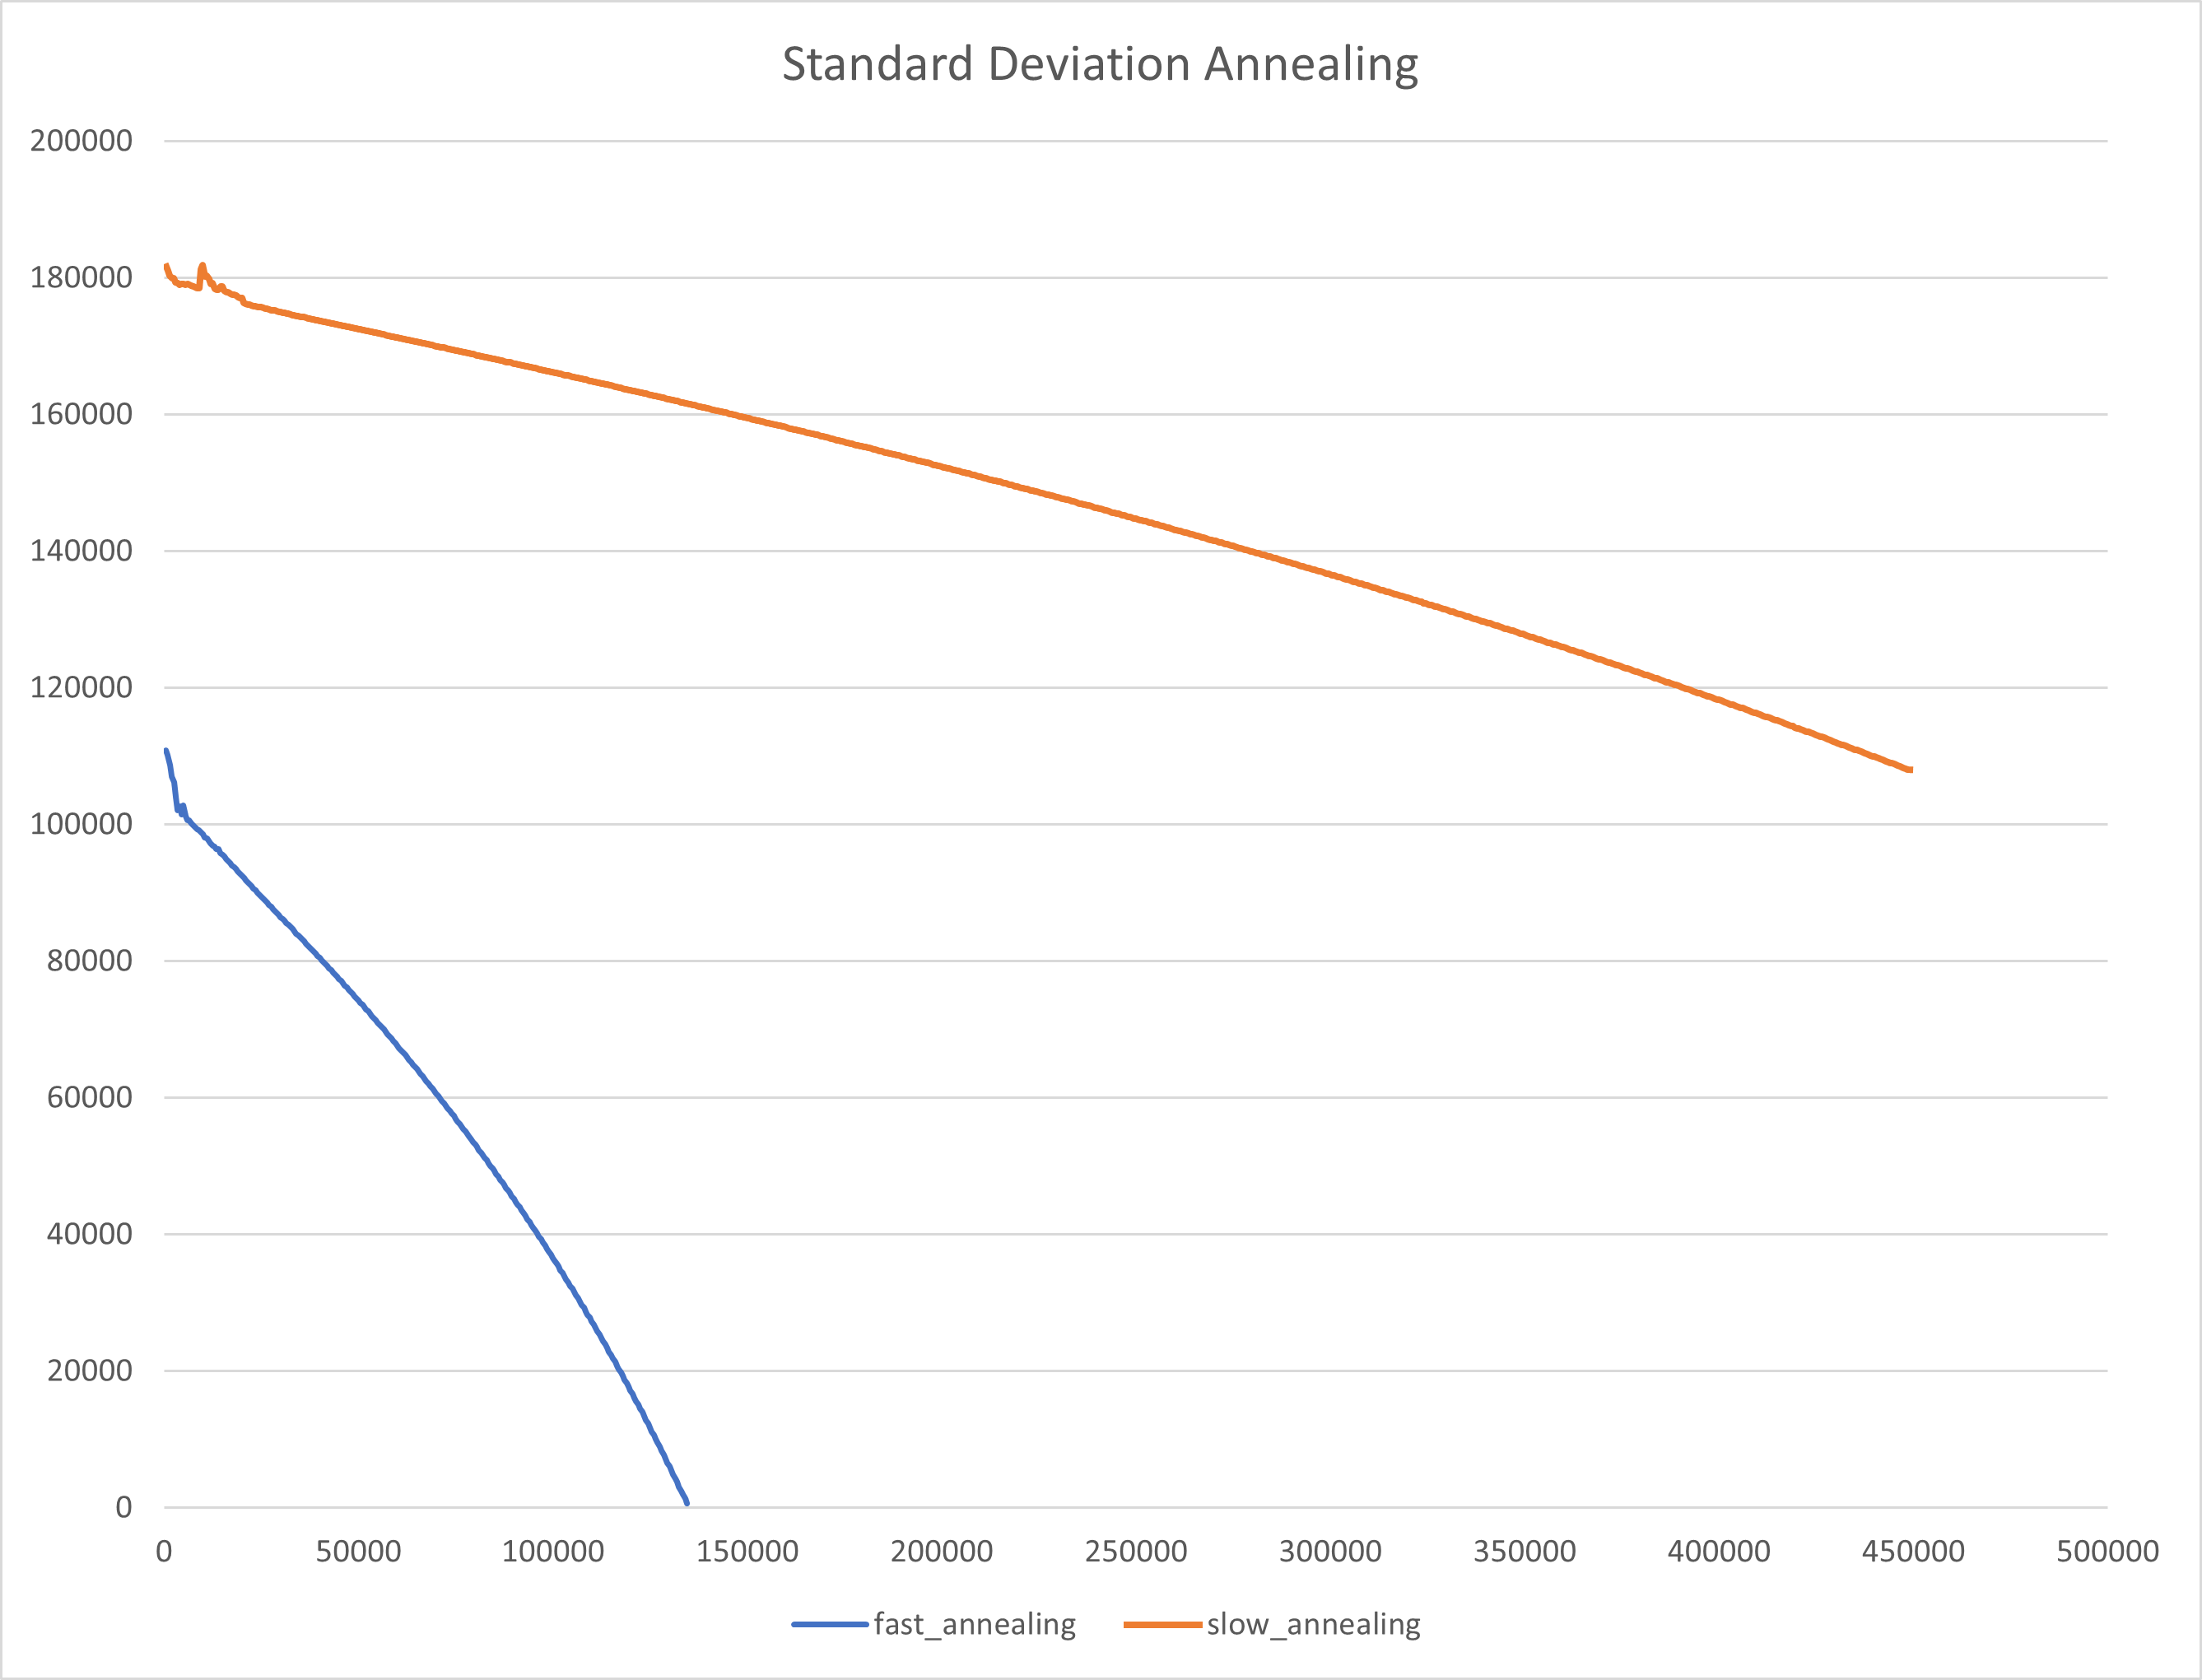
\includegraphics[width=.5\linewidth]{STD_Annlng.png}
    \caption{Change in loss value due to fast and slow annealing of standard deviation}
    \label{fig:stdannl}
\end{figure*}


\begin{equation}
\begin{aligned}
  f_t =& \sigma(W_f \ast x_t + V_f \ast h_{t-1} + U_f \circ c_{t - 1}\\ 
         & + b_f)\\
  i_t =& \sigma(W_i \ast x_t + V_i \ast h_{t-1} + U_i \circ c_{t - 1}\\ 
         &  + b_i)\\
  o_t =& \sigma(W_o \ast x_t + V_o \ast h_{t-1} + U_o \circ c_{t - 1},\\
         & + b_o),
\label{eq:LSTMFC}
\end{aligned}
\end{equation}

where "$\ast$" denotes the convolution operator and "$\circ$" denotes the Hadamard product. In my implementation, I removed the peephole connection in each gate. The equations \ref{eq:LSTMFC}become as follows:

\begin{equation}
\begin{aligned}
  f_t =& \sigma(W_f \ast x_t + V_f \ast h_{t-1} + b_f)\\
  i_t =& \sigma(W_i \ast x_t + V_i \ast h_{t-1} + b_i)\\
  o_t =& \sigma(W_o \ast x_t + V_o \ast h_{t-1} + b_o)
\label{eq:LSTM}
\end{aligned}
\end{equation}

\subsubsection{Loss calculation} \label{sec:losscalc}

The model is trained using a loss function called the Evidence Lower BOund (ELBO) loss. This training process aims to learn the embedding vector $r$ \cite{2013arXiv1312.6114K}. The Kullback-Leibler divergence (KL-D) term constrains the learning process. This term measures the difference between the approximation of the learned distribution (the distribution of latent variable $z$ given the encoded latent variable $Q(z|h_{enc})$) and a prior standard Gaussian distribution, which has a mean of zero and a variance of one ($\mathcal{N}(0,1)$).

In my implementation of the model, the KL-D term is not compared to the standard Gaussian distribution ($\mathcal{N}(0,1)$), but rather to the prior distribution of latent variable $z$ ($p(z)$). Additionally, in the original version of the model, the reconstruction loss is calculated based on the assumption that the output distribution follows a Bernoulli distribution. In my implementation, the reconstruction loss is calculated, assuming that the output follows a normal distribution. See Section \ref{sec:training} for more discussion about why I used the Normal distribution instead of the Bernoulli distribution.

\subsubsection{Model Hyperparameters}

The transformer encoder consists of a stacked four-layers encoder. Each encoder layer has a four-head self-attention block with a hidden size of 64 and a position-wise feed-Forward block with an inner layer with dimensionality ($d_{ff}$) of 200. The embedding layer has an output size of 64 and is initialized by 42B-token, 300d Glove pre-trained vectors \cite{pennington-etal-2014-glove}. All other parameters are the same as the original model. 

\subsection{Training} \label{sec:training}

The model is originally trained using the ADAM optimizer with a learning rate starting at $5e-5$ and linearly decayed to $5e-4$ over one million steps. I trained the model with the same learning rate for the image generation part; however, for the transformer language encoder, I used a faster learning rate that started at $1e-3$ and linearly decayed to $5e-4$ over one million steps. I used a faster learning rate for the transformer because the model training is highly demanding in terms of computational requirements hoping that the model will converge faster. Also, to speed up the training time, I calculate the reconstruction loss assuming that the output follows a normal distribution. By doing so, I can fast anneal the loss function's standard deviation by starting with a high standard deviation and gradually decreasing it over time. In my implementation, I started with a standard deviation of $1.0$ then and linearly reduced it to $0.1$ over $2e5$ steps. Figure \ref{fig:stdannl} shows the difference in the training time between the used annealing  and a slower configuration that started with a standard deviation of $2.0$ then and linearly reduced it to $0.1$ over one million steps.


\begin{figure*}[t]
    \centering
    \begin{subfigure}[]{0.49\textwidth}
        \centering
        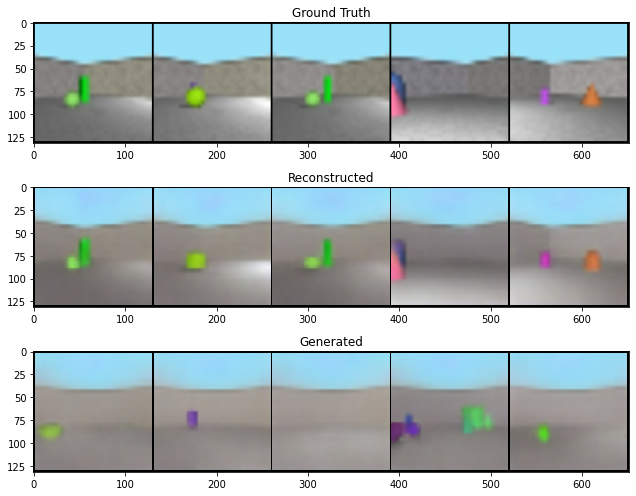
\includegraphics[width=\textwidth]{output1.png}
        \caption{}
        \label{fig:output1}
     \end{subfigure}
     \begin{subfigure}[]{0.49\textwidth}
        \centering
        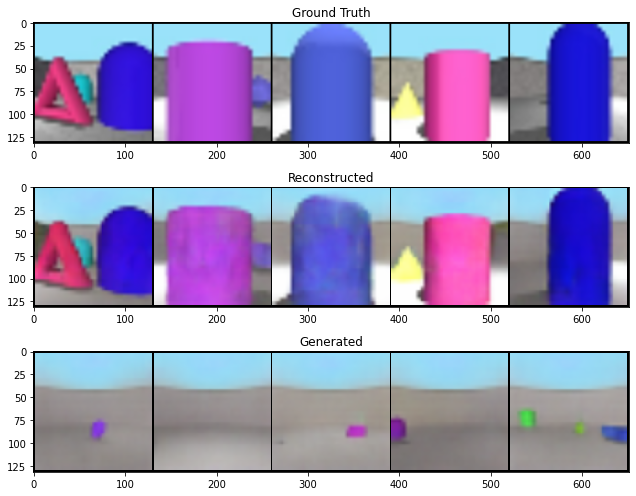
\includegraphics[width=\textwidth]{output2.png}
        \caption{}
        \label{fig:output2}
     \end{subfigure}
    \caption{Ground truth images (first row), reconstructed images (middle), and generated images (last raw). (a) shows the best five images with the lowest reconstruction loss, while (b) shows the images with the highest reconstruction loss.}
    \label{fig:outputs}
\end{figure*}

\subsection{Experiments}

The model is tested against a separate test dataset using the following approaches:

\paragraph{Training-like process:} In this approach, I passed the input images through the VAE's model (including the encoder and decoder networks) to obtain the predicted output. This approach is similar to the process used during training and allows you to see how well the model can reconstruct the input images.

\paragraph{Generation process:} In this approach, I sampled a latent space from a normal distribution with a mean of zero and a standard deviation of one and passed it through the VAE's decoder network to obtain the predicted output.

\section{Results and discussion}

\paragraph{Images reconstruction:} Figure \ref{fig:outputs} shows the experiment's results. The figure shows that the images (with the lowest and highest loss) are reconstructed well. This result indicates that the model can reconstruct the input images. 

\paragraph{Samples generation:} However, the model cannot generate new samples by sampling latent codes from the normal probability distribution. One notices that the model cannot generate the proper objects and can generate the room walls. The ability of the model to reconstruct the input images and its failure to generate new samples indicates that the model fails to encode the underlying structure of the images, and it learns only the room. This generation's failure may be due to my choice to speed up the training process because the model did get a suitable level of variability to assign values to the reconstructed data; the model cannot "explore" a wider range of values. 

\paragraph{Text Embedding:} Talking about the language part is problematic because of the failure of the generation network.

\section{Future Work}

After properly model training, the following tests could be done:

\paragraph{Semantic coherence analysis:} the authors examined how well the language representation is semantically consistent. They applied several sentence transformations on the base sentences in the test dataset. Then they measure the similarity between each base sentence representation and its transformations representation using the cosine distance. The transformations used are noun change, adjective change, preposition change, and meaning preservation. 

In addition to using cosine distance, the transformer encoder's self-attention could be examined. Also, as the images are relatively simple; there are eight shaps, six spatial relations, three adjectives for sizes, and twenty-two  colors, an automatic algorithm could be developed to compare the transformed sentences with the generated images.

\newpage
\bibliography{acl2020}
\bibliographystyle{acl_natbib}



\end{document}
